\documentclass{article}
\usepackage{fancyhdr}
\usepackage{extramarks}
\usepackage{amsmath}
\usepackage{amssymb}
\usepackage{enumerate}
\usepackage{graphicx}
\usepackage{pgfplotstable}
\usepackage{listings}
\usepackage{braket}
\usepackage{float}
\usepackage{subfig}
\lstset{framexleftmargin=5mm, frame=shadowbox, rulesepcolor=\color{blue}}


\topmargin=-0.45in
\evensidemargin=0in
\oddsidemargin=0in
\textwidth=6.5in
\textheight=9.0in
\headsep=0.25in

\linespread{1.1}

\pagestyle{fancy}
\lhead{Chase Brown}
\chead{Solid State Physics : Study Notes}
\rhead{\firstxmark}
\lfoot{\lastxmark}
\cfoot{\thepage}

\renewcommand\headrulewidth{0.4pt}
\renewcommand\footrulewidth{0.4pt}

\setlength\parindent{24pt}

	

\begin{document}

	\section{Solve Graphene/Graphite Diffraction Scattering, Construct Brillouin Zone, solve for band structure with $k\cdot p$, tight binding, free electron, and nearly free electron theory}
		
		It was mentioned in class that a scattering problem would be presented on the final as well as a BZ solving problem.  		
			
		\subsection{Constructing the BZ}
			To construct the BZ you must:
			\subsubsection{Draw the reiprocal lattice}
				\textbf{Simple Cubic}

					Starting with the lattice for a SC structure shown below (real space) we can construct the reciprocal lattice.
				

					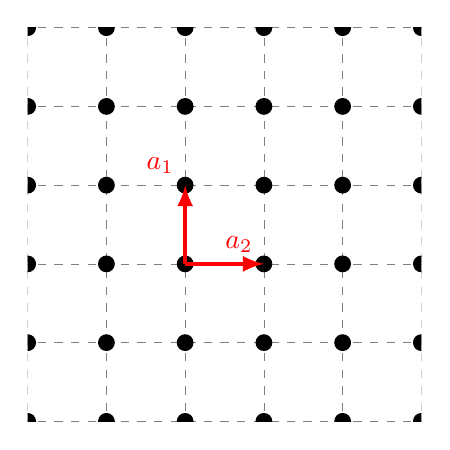
\begin{tikzpicture}
					\begin{scope}
					\clip (0,0) rectangle (5cm,5cm); % Clips the picture...
					\draw[style=help lines,dashed] (-14,-14) grid[step=1cm] (14,14); 
					
					\foreach \x in {-7,-6,...,7}{
					    \foreach \y in {-7,-6,...,7}{ 
						    \node[draw,circle,inner sep=2pt,fill] at (\x,\y) {}; 
    						}
					}
					
					\draw [ultra thick,-latex,red] (2,2) -- (2,3) node [above left] {$a_1$};
					\draw [ultra thick,-latex,red] (2,2) -- (3,2) node [above left] {$a_2$};
					\end{scope}
					\end{tikzpicture}
				
									

			\subsubsection{Construct the Brillouin Zone}

			
	\section{Understand and solve for the Raman spectroscopy output from a graphene sheet}
		

\end{document}
